\chapter{A model of PME in multiply-connected superconductors}
\label{chap:pme_theory}

\section{Introduction}

As discussed in the chapter \ref{chap:pme_experiment}, there have 
been many previous observations of PME in superconductors. 
In addition to these experimental observations, there 
have also been several attempts to describe a model for 
the PME in these superconductors. 

\subsection{\pijunction\ models}

The first attempt to describe PME in \hightc\ came from
Sigrist and Rice \cite{sigrist_jpsj_61_4283_1992,%
sigrist_rmp_503_67_1995}\ who argued that the presence 
of \pijunctions in a superconductor would cause it to be
paramagnetic. They further argued that \pijunction s would
come about due to a \dwave\ order parameter coupled with
misaligned grains in the superconductor. This idea is basically
the single loop model as discussed in chapter \ref{chap:jjarray}
(section \ref{sec:single_loop}, p. \pageref{sec:single_loop}, 
\EqnRef{eqn:steadystatepijunction}).
It was discussed that Sigrist and Rice chose a value of 
\betal\ that was too small. Had they chosen a larger value
of \betal\ they would have seen that paramagnetism would be 
possible at $\phiext=0$, for a loop with no \pijunctions\, 
a phenomena which they attributed
to the presence of a \pijunction\ in the loop. It should be noted
that Sigrist and Rice proposed this theory before the first
observation of PME in \lowtc\ superconductors\cite{thompson_prl_75_529_1995}.

Because the Sigrist and Rice work was based on the idea of a 
single superconducting loop, others began to try and model the
superconductor as various types of \jjas. One model
was carried out by Dominguez \etal\cite{dominguez_prl_72_2773_1994}
but contained several flaws. They treat the case of a \jja\ with 
randomly distributed \pijunctions, but do not treat they case of an
array without \pijunctions. This failing is similar to that of 
Sigrist and Rice, and they reach the similar conclusion that 
the presence of \pijunctions\ make the sample behave 
paramagnetically. 

\subsection{\jja\ models}

Similar models of this
type were carried out by Auletta \etal\cite{auletta_prb_49_12311_1994}
who modeled the array as a series of concentric loops of \jjsnoun\  
with mutual
inductance. Additionally, Chandran\cite{chandran_prb_56_6169_1997}
performed similar calculations using a square array and a full
mutual inductance matrix. 
Both Auletta \etal\ and Chandran use 
simplified models for the \jjsnoun\
which ignore the capacitance of the
junction (RSJ model). 
Additionally, both treat only the case of no \pijunctions, 
alleviating the problems with the Sigrist and Rice and the Dominguez \etal\
models. 
Remarkably, however, they are able to recreate the 
temperature dependent magnetization during a field cooling experiment. 
Unfortunately, neither report on the spatial distribution of the
magnetization over the array, which is what we have measured directly
here. 

More recently, De Leo \etal\cite{deleo_unpublished}, modeled 
an RCSJ \jja\ dynamically through the field-cooling process, and 
obtained results remarkably similar to those discussed in 
chapter \ref{chap:pme_experiment}. The relationship between this model
and the experiment will be discussed in more detail in section
\ref{sec:num_array_sims}. 

\subsection{Flux compression}

In a departure from the \jja\ model of PME there have been other
proposed models. Koshelev and Larkin\cite{koshelev_prb_53_13559_1995}
proposed the so-called flux compression model. \index{flux compression}
The flux compression model relies on the superconductor having a 
spatial variation in $T_c$, such that the exterior of the sample
becomes superconducting before the interior of the sample, through
either a differential cooling or a spatial distribution of 
$T_c$. Because the exterior becomes superconducting first, it 
effectively traps flux in the center of the sample, and compresses
the trapped flux (hence ``flux compression'') as the 
superconducting region grows
from the outside-in. This trapped flux, and the
screening currents required to keep the flux trapped, create
a positive magnetic moment, the paramagnetic Meissner effect.
An interesting aspect of the flux compression model is that it gives
specific predictions for the flux and current distribution
throughout the sample -- something that can easily be tested with
the SQUID microscope. 

A phenomena related to the flux compression model is the ``giant
vortex state'' model\cite{moshchalkov_prb_55_11793_1999,%
deo_prl_79_4653_1997} which is appropriate for mesoscopic
superconductors, such as the Al disks measured by Geim \etal\
\cite{geim_nature_396_144_1998}, but does not apply to the 
macroscopic situations discussed here. 

\subsection{Pinning and surface barriers}

In addition there are other proposed models which essentially rely
on defects in the superconductor to create the PME. 
One may imagine, \eg\, that surface damage to the superconductor
pins flux during the field cooling process 
and causes the sample to be paramagnetic. It has
additionally been proposed that some type of surface barrier
may result in flux trapping in the sample\cite{deo_prb_59_6039_1999},
or that 
Andreev bound states at the
surface of the superconductor\cite{prusseit_physc_317_396_1999}
may result in paramagnetism. 

\section{Experimental comparison to various models}

It has already been stated that the simple models involving \pijunctions\
do not reflect reality in the \jja\ samples that were measured. 
It has clearly been demonstrated that Nb, an \swave\ superconductor,
exhibits PME in the absence of \pijunctions. Furthermore, it is
clear from the discussion of the single loop in chapter \ref{chap:jjarray}\
that a single loop of \jjsnoun, without any \pijunctions, can in
theory be paramagnetic after field cooling. 

The various models treating PME in an array model of superconductivity
have great merit, but do not provide any spatially resolved data
to which we might compare our array data.

Based on our experimental observations we can clearly rule out
the flux compression model as untenable. Our data looks nothing
like the proposed flux distribution for a sample exhibiting
flux compression. Furthermore, we do not expect any of the 
requirements of flux compression to be met in our experiment. 
Our sample is well grounded thermally to the sapphire rod of the
sample stage in the experiment. Furthermore because of the
photolithographic uniformity
we do not expect that the outermost islands of the 
array would have a $T_c$ \emph{higher} than the inner islands. 
If anything we would expect deposition errors to cause the edge 
islands to have defects
which would tend to 
\emph{lower} the $T_c$. 

Indeed, the primary features of our experimental data are not
predicted by any of the known theories of PME. We always observe a
diamagnetic region around the edge of the sample in addition to 
a region of Gaussian distributed flux inside, but generally with
a  paramagnetic mean. Finally the paramagnetism of the array increases
with increasing external field. 

\section{Array screening}

The presence of the diamagnetic screening current flowing around
the outside edge of the array must be accounted for in any 
realistic model. The array could possibly accomplish this diamagnetic
screening in one of two ways. 

\begin{figure}
\includegraphics[width=5.0in]{figs/pme_theory/fig41.eps}
\caption[Comparative array screening: individual plaquette \vs\ 
large outside loop]
{Comparative ways to generate Meissner screening in an array.
(a) A large loop of many \jjsnoun\ around the outside edge of the
array. (b) Each plaquette single screening flux from the interior
of itself, and hence screening from the entire array. }
\label{fig:comp_array_screening}
\end{figure}

First, the array may generate a screening
current flowing around the outside edge of the array; in effect
creating a large loop of $2(N + M)$ junctions around the outside
of the array. 
\MultFigRef{fig:comp_array_screening}{a}\ depicts this situation. 
This picture is similar to how a bulk 
superconductor might screen, with current flowing just around the outside
edge and nowhere else inside. 
We can quickly see that this
large loop can screen a maximum external field of 
$B_{\mathrm{max}}=\Phinot \betal /2 \pi a^2 (NM)^{1/2}$. This
maximum field shrinks as the size of the array, $NM$, increases.

The second possibility, depicted in 
\MultFigRef{fig:comp_array_screening}{b}\ is that each plaquette 
may screen flux from 
itself. In this case, each plaquette may screen up to 
$B_{\mathrm{max}} = \Phinot \betal /2 \pi a^2$. 
In this picture, flux will not penetrate the array until flux
is able to penetrate a single plaquette. The maximum
field in this case is always greater, and substantially greater
for large arrays, than for the single loop, making this difference
quite easy to discern experimentally. 

One clear way to think about these two configurations is to realize 
that in both cases, the maximum current that may flow around any 
current path is $I_c$. Presented here are the two limiting cases. 
In the large loop current case, the maximum field is screened with
$I_c$ flows around the entire array. In the second case, the maximum
flux may be screened when $I_c$ flows around a single plaquette. 
It is clear that the amount of flux that flows through the enclosed
area, due to the currents, is far larger in the latter case than
in the former. 

Indeed, 
AC susceptibility measurements by Araujo-Moreira \etal
\cite{araujo_prl_78_4625_1997} demonstrated this, in arrays of the 
same geometry as those discussed here. They showed that 
the array did not respond hysteretically to a driving external field
until the amplitude of the external field was increased above approximately
$4\,\Phinot$ per unit cell. For the $\betal =30 $ used here this
indicates that single
plaquettes of the array are screening.  

Furthermore, we have observed flux penetration into our array in the
Meissner state and noticed that the flux does not penetrate until the
external field is ramped from zero to exceed $4\,\Phinot$ per unit cell
of the array. An example of this penetration is shown in 
\FigRef{fig:init_flux_penetration}. The figure shows the first
flux penetration into the array at a field of $4.8\,\Phinot$ per unit cell 
of the array. Notice that the flux penetrates as fingers, apparently
nucleating from a single plaquette, indicating that it was the screening
of a single plaquette that broke down (perhaps due to a weak $J_c$) 
and allowed flux to penetrate. 

\begin{figure}
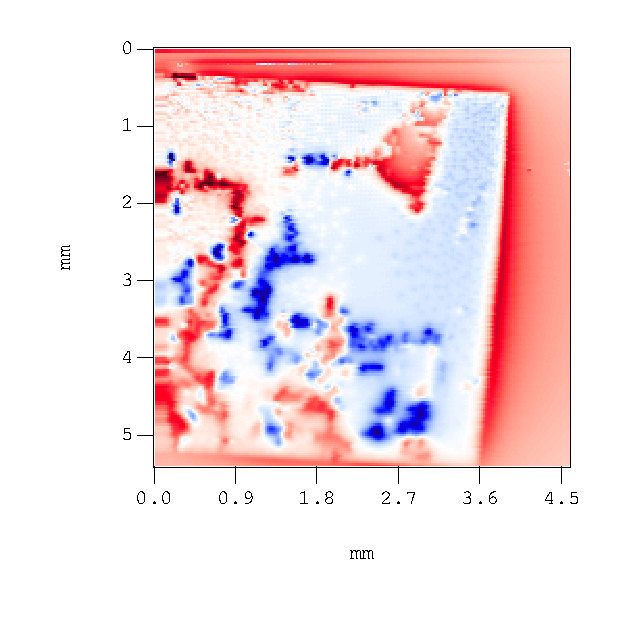
\includegraphics[clip=true]{figs/pme_theory/fig42.eps}
\caption[Initial flux penetration into \jja]{Initial flux 
penetration into \jja\ at an external field of 4.8 \Phinot.}
\label{fig:init_flux_penetration}
\end{figure}

\subsection{Outer diamagnetic current}

The previous section demonstrated that the each plaquette of the array
screens flux from itself, rather than the entire array 
screening by way of a large current loop around the outside edge
of the array. 
However, it was observed 
(\cf\ \FigRef{fig:paramag_image}(a) and (c) ) in all of the 
cooling images that the array always generated a diamagnetic 
screening current around the outside edge. To
generate an overall diamagnetic screening current,
and have each plaquette screening individually, one may think
that they array constructs a picture as in 
\MultFigRef{fig:plaquette_screening}{a}, in which all the 
internal currents of the array cancel to generate an overall
diamagnetic current. 

\begin{figure}
\includegraphics[width=5.0in]{figs/pme_theory/fig43.eps}
\caption[Different array screening configurations for individual
plaquettes]
{Possible different array screening configurations. (a) Every
plaquette of the array screening. (b) Only the outside edge plaquettes
of the array screening. }
\label{fig:plaquette_screening}
\end{figure}

However, it may not be true that the currents cancel. For our array
geometry, the array wire width is $10\,\micron$, but the penetration
depth of niobium at $4.2\,\kelvin$ is $900\,\angstrom$. This means that
the internal currents of the array will not cancel. Instead currents
flow internal to the array around each plaquette. 
\FigRef{fig:plaquette_screening_close_up} schematically demonstrates
this situation for two neighboring plaquettes. 
Because of the discrepancy between the wire width
and the penetration depth of niobium, the internal currents do not
cancel. Instead each screening loop of the array must generate 
a current flowing around the plaquette. 

\begin{figure}
\includegraphics[width=5.0in]{figs/pme_theory/fig44.eps}
\caption[Close up view to two adjacent screening plaquettes]
{Close up view of two adjacent screening plaquettes. The geometry
is for our array. The wire width is $10\,\micron$ and the penetration
depth for niobium is $900\,\angstrom$. Because of this discrepancy,
the internal currents do not cancel, as shown, and the array
must actually generate a loop of current flowing around each
plaquette}
\label{fig:plaquette_screening_close_up}
\end{figure}

% currents canceling in overlap geometry junctions. 
It is argued above that 
the internal currents to the array do not cancel within the wires. 
It turns out that in the overlap \jjnoun\ geometry the current
flowing through the \jjnoun\ spreads out uniformly so we expect
the currents flowing through the junctions to cancel, and not
give a contribution to the net Josephson energy. 

To generate this configuration we find that the energy stored
magnetically due to all the plaquette current loops in the array 
is
%
\begin{equation}
E_{\mathrm{mag}} = NM\, \frac{1}{2} LI^2.
\end{equation}
%
Additionally, there is a Josephson energy contribution to the energy
from the junctions around the outside edge of the array
%
\begin{equation}
E_J = 2(M+N)\, E_J (1-\cos\gamma)
\end{equation}
%
This leads to a total energy of 
%
\begin{equation}
E_{\mathrm{tot}} =  NM \,\frac{1}{2} LI^2 + 
          2(M+N)\, E_J (1-cos\gamma).
\label{eqn:all_loop_screening}
\end{equation}
%
This total energy grows as $N\times M$, and for a large array can be quite 
substantial. 

It turns out that it is possible to create a screening mechanism, in
which the total array energy grows as $N+M$. 
This screening configuration is shown in 
\MultFigRef{fig:plaquette_screening}{b}. Here only the plaquettes on 
the outside edge of the array screen. This creates the observed external
diamagnetic screening current. But we end up with a total magnetic
energy of 
%
\begin{equation}
E_{\mathrm{mag}} = 2(N+M)\, \frac{1}{2} LI^2.
\end{equation}
% 
Additionally, there is a contribution due to the Josephson energy
in the outside edge junctions, but also due to the edge 
junctions just inside the screening plaquettes, as shown in 
\MultFigRef{fig:plaquette_screening}{b}. 

in the inside edge junctions
%
\begin{equation}
E_J =\left\{ 2(N+M) + 2(N + M - 2) \right\}\, E_J (1-\cos\gamma),
\end{equation}
%
yielding a total energy of 
%
\begin{equation}
E_{\mathrm{tot}} = 2(N+M)\, \frac{1}{2} LI^2 +
 \left\{ 2(N+M) + 2(N + M - 2) \right\}\, E_J (1-\cos\gamma).
\label{eqn:edge_loop_screening}
\end{equation}
%
This energy is smaller than the energy in the previous case
in which all of the plaquettes screen. As the size of the array
grows, this energy becomes more favorable (\cf\ $N+M$ \vs\ $N\times M$).

Comparing \EqnRef{eqn:all_loop_screening}\ and 
\EqnRef{eqn:edge_loop_screening}\ and assuming that $\gamma$ is 
proportional to $\Phitot$ and $N=M$
we deduce that it will be energetically
favorable for the array to screen with only the outside when,
%
\begin{equation}
\betal > {4 N -1 \over N^2 - 4N}
\end{equation}
%
which is valid for all $N>2$. For the arrays we consider, this 
criteria is easily satisfied. 

\section{Consequences of edge loop screening}

In the second case, with only the edge loops screening, 
in addition to the diamagnetic screening current flowing immediately
around the outside edge, there also is a paramagnetic
current flowing just inside the outside edge. This paramagnetic
current is closer to the interior of the array than the diamagnetic
current. The interior plaquettes of the array will respond to both
the diamagnetic current and the paramagnetic current, but the 
paramagnetic current is closer to the interior plaquettes, so 
it will dominate the response of the interior plaquettes. 
\FigRef{fig:screening_schematic}\  schematically shows this situation, 
depicting the external diamagnetic screening current and the interior
paramagnetic current.

\begin{figure}
\includegraphics[width=5.0in]{figs/pme_theory/fig45.eps}
\caption[Schematic of interior and exterior plaquettes, with screening
provided by external plaquettes only]
{Schematic of interior and exterior plaquettes, with screening provided
by external plaquettes only. The diamagnetic screening current flows 
around the outside edge of the array, while the paramagnetic current
flows just inside the edge of the array.}
\label{fig:screening_schematic}
\end{figure}

\subsection{Single loop response to external field shift}

Each interior plaquette essentially sees a shift in the external field
applied to it, due to the diamagnetic and paramagnetic currents
discussed above. 
We must consider the effect of these two currents to the 
single loop's magnetization before continuing. The external flux
that each interior plaquette sees is the real external flux, 
plus a contribution due to the external currents
%
\begin{equation}
\Phiext -> \Phiext + \Phi_{\mathrm{screen}}.
\label{eqn:ext_flux_redef}
\end{equation}
%
If we apply this modification to the magnetization relation for a 
single loop, shown in \FigRef{fig:single_loop_mag}, we see that the
entire magnetization curve for the single loop is shifted upward
so that the single loop will more often appear to be 
\emph{paramagnetic}. It must be pointed out here that this 
shift is really just a book-keeping shift, because of the 
redefinition of the external flux that affects the single 
loop, \EqnRef{eqn:ext_flux_redef}. 

\subsection{Array response to external shift}

We computed the $\Phi_{\mathrm{screen}}$ term
over the entire interior of the array
for the geometry of the $30 \times 100$ array;
determined the shift in the magnetization of each interior
plaquette; and found that the 
minimum induced magnetization occurs in the central plaquette of
the array and is approximately $\Phimag=0.15\,\Phinot$. Furthermore,
we can determine the average induced magnetization over the 
entire interior of the array, and determine it to be 
$\Phimag=0.27\,\Phinot$. These numbers compare favorably with the observed
average
magnetization numbers seen in the array (\cf\ \FigRef{fig:sm_array_mag_plot}).

Of course, this simple model does not capture many other important
features experimentally observed in the array. It does not explain
\eg\ the apparent random distribution of flux over the interior of the
array. Quite the contrary, it predicts that the paramagnetism should
be strongest near the edges of the array, and weakest in the center
of the array. Furthermore, this simple model predicts that they array
interior
should be entirely paramagnetic while it we observe that there
are diamagnetic regions in the array interior. 

\subsection{Numerical array simulations}
\label{sec:num_array_sims}

Fortunately, numerical simulations of an array system similar to ours,
using the RCSJ model for the entire array (\cf\ chapter \ref{chap:jjarray},
section \ref{sec:entire_array_model}, p. \pageref{sec:entire_array_model}
and  Eqns.~(\ref{eqn:junc_horiz}) to 
(\ref{eqn:total_flux_array})) have been carried out recently%
\cite{deleo_unpublished} and obtain results that replicate quite
well the experimentally observed flux distribution in the array.

In this numerical experiment, De Leo \etal\ take a $10\times 40$ 
\jja\ and model the experiment by increasing \betal\
and \betac\ from zero to their final values at $T=4.2\,\kelvin$
to simulate the field cooling process. After waiting for
transient solutions to decay, a steady state solution is arrived 
at for the array. 

\begin{figure}
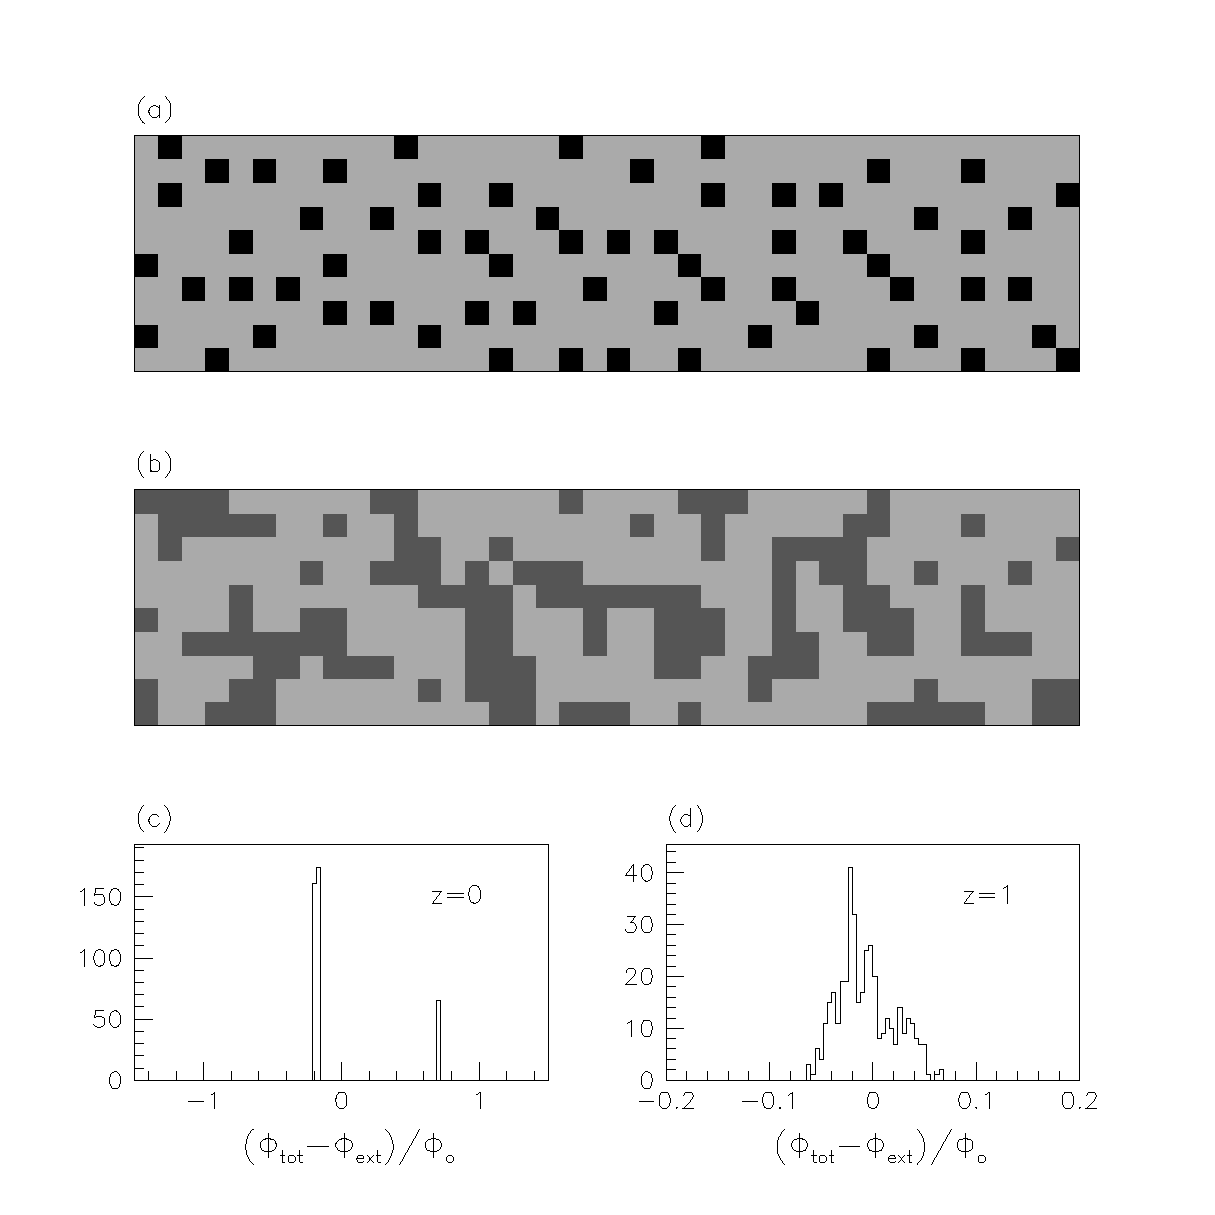
\includegraphics[width=5.0in]{figs/pme_theory/fig46.eps}
\caption[Modeled array magnetization for a $10\times 40$ \jja,
field cooled in $\phiext = 4.8$]
{Modeled array magnetization for a $10\times 40$ \jja, field
cooled in $\phiext = 4.8$. 
Red represents paramagnetic plaquettes and blue represents
diamagnetic plaquettes.
(a) The array magnetization at the surface of the array. 
(b) The array magnetization as measured at a height of one
unit cell above the array. 
(c) Histogram of the array magnetization at the surface of the
array.
(d) Histogram of the array magnetization at a height of one
unit cell above the array. }
\label{fig:model_array_mag}
\end{figure}

\FigRef{fig:model_array_mag}\ shows the results of the field
cooling simulation for a $10 \times 40 $ \jja. Red colors represent
paramagnetic plaquettes and blue colors represent diamagnetic 
plaquettes. \MultFigRef{fig:model_array_mag}{a}\ shows the 
magnetization as measured at the surface of the array, and
\MultFigRef{fig:model_array_mag}{c}\ shows a histogram of the
same data. The spatial distribution of the magnetization in (a)
is very suggestive of the data as we measured (\cf\ 
\FigRef{fig:paramag_image}). However, the histogram in 
\MultFigRef{fig:model_array_mag}{c} is quite different from that
measured in \MultFigRef{fig:paramag_image}{b}. What's truly
striking about  \MultFigRef{fig:paramag_image}{b}\ however, is that
the two peaks correspond almost exactly to the lowest and second
lowest Gibbs free energy solutions for the single loop
(\cf\ chapter \ref{chap:jjarray}, section \ref{sec:gibbs_free_energy},
p. \pageref{sec:gibbs_free_energy}). Perhaps more interesting is
\MultFigRef{fig:model_array_mag}{b}\ which shows the simulated
magnetization of the $10 \times 40 $ array at a height of one 
plaquette. This is similar to the magnetization that a SQUID might
measure at a height of one plaquette. Indeed the SQUID in our 
experiments was at a height of approximately one plaquette. 
Interestingly, the histogram shown in \MultFigRef{fig:model_array_mag}{d}\
closely resembles the experimental histogram in 
\MultFigRef{fig:paramag_image}{d}.

Furthermore, De Leo \etal\ modeled the external field dependence of the 
array magnetization, shown in \FigRef{fig:sim_array_mag}. Their results
qualitatively resemble the results obtained in \FigRef{fig:sm_array_mag_plot}\
providing good evidence that the properties of our array can be replicated
simply from the equations describing a \jja. 

\begin{figure}
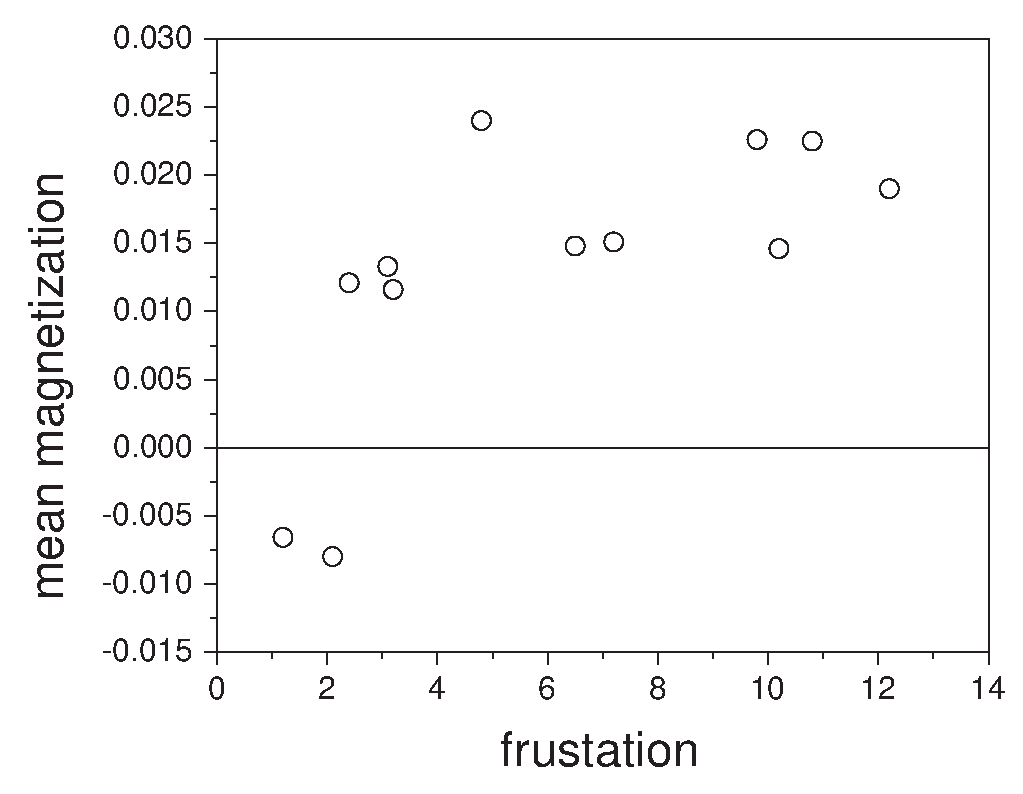
\includegraphics[width=5.0in]{figs/pme_theory/fig47.eps}
\caption[Simulated array magnetization \vs\ cooling field]
{Simulated array magnetization \vs\ cooling field for the 
$10\times 40 $ \jja.}
\label{fig:sim_array_mag}
\end{figure}
